\chapter{Implementação do Processo}
\label{chap:capacitor}
% ----------------------------------------------------------
Este capítulo apresenta a implementação do
Processo de Avaliação de Capacidade descrito no capítulo anterior, bem como da técnica de
Inferência de Desempenho e das Heurísticas de Seleção que dão suporte a esse
Processo. A implementação está estruturada na forma de uma biblioteca
extensível, denominada CloudCapacitor, e de um sistema computacional que demonstra seu funcionamento, denominado Capacitor Web. 

%Foi dado o nome de CloudCapacitor à biblioteca, implementada como uma \emph{gem}
%(i.e., um pacote) da linguagem Ruby~\cite{ruby} e desenvolvido o sistema
%computacional Capacitor Web para ser uma interface visual para a utilização do CloudCapacitor, usando 
%o \emph{framework} Ruby on Rails~\cite{rails}.  

A seguir são descritos os detalhes da implementação de cada um destes módulos e
como ambos se relacionam para oferecer ao usuário a experiência da avaliação de capacidade
de baixo custo e alta precisão prevista pelo Processo proposto, com uma interface
amigável e de fácil utilização.

\section{CloudCapacitor}
CloudCapacitor é uma biblioteca para criação de sistemas de avaliação de 
capacidade em ambientes de nuvem IaaS, implementada como uma \emph{gem}
(i.e., um pacote) da linguagem Ruby~\cite{ruby}. A biblioteca fornece uma implementação
completa da especificação do Processo de Avaliação de Capacidade descrito no 
Capítulo~\ref{chap:processo}, permitindo que sejam customizadas as atividades 
definidas como pontos de extensão do Processo, como as Estratégias de Avaliação
e a execução da Aplicação sob Teste.

Primeiramente, serão apresentadas as classes que compõem a biblioteca
e suas responsabilidades. Em seguida, será mostrado como CloudCapacitor auxilia 
desenvolvedores de software na criação de sistemas de avaliação de capacidade,
mostrando o fluxo de utilização da biblioteca através de sua interface de programação.
Depois, serão explicados alguns detalhes de implementação da biblioteca, como 
a solução para representação do Espaço de Implantação e seu papel na execução do
Processo de Avaliação de Capacidade. Por fim, serão apresentados os pontos de extensão
da biblioteca, notadamente como implementar um Executor, a classe responsável pelo
controle de execução da Aplicação sob Teste, e como sobrescrever a Estratégia de
Avaliação fornecida pela biblioteca a fim de alterar seu comportamento padrão.

Para concluir a apresentação do CloudCapacitor, será mostrada a saída de dados
fornecida pela biblioteca com as Configurações capazes de executar a
Aplicação sob Teste em cada uma das Cargas de Trabalho respeitando o SLA definido.

\subsection{Classes e Responsabilidades}
\label{subsec:classes}
A biblioteca CloudCapacitor é formada por um conjunto de classes que representam os
componentes envolvidos na avaliação de capacidade de aplicações em ambientes de
nuvem de acordo com os conceitos e o Processo definidos anteriormente, no
Capítulo~\ref{chap:processo}. A Figura~\ref{fig:classes}
mostra as principais classes cujas responsabilidades e cooperação levam ao 
resultado final de uma Avaliação. 

Ao utilizar a biblioteca CloudCapacitor na construção de um software para avaliação
de capacidade, o desenvolvedor tem à sua disposição uma classe principal, chamada
\emph{Capacitor}. Essa classe fornece o fluxo principal do Processo de
Avaliação, com todos os seus pontos de decisão e de extensão.

\begin{figure}[t]
  \begin{center}
    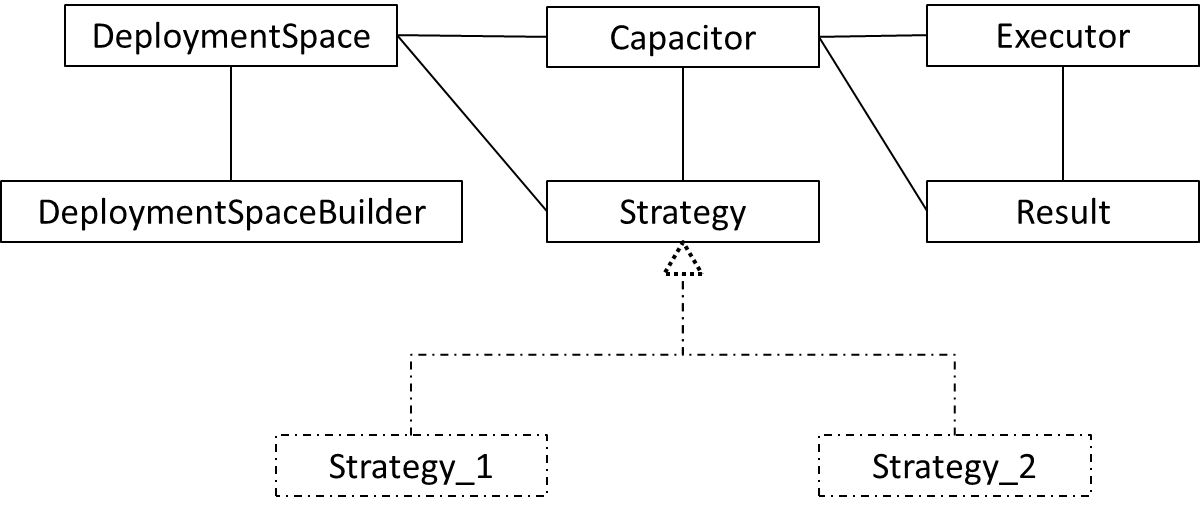
\includegraphics[scale=0.65]{img/CapacitorClasses}
  \end{center}
  \caption{\label{fig:classes}Principais classes que compõem o CloudCapacitor e suas relações.}
\end{figure}

Entre os pontos de extensão, destaca-se o uso da classe \emph{Strategy}. Como 
pode ser visto na Figura~\ref{fig:classes}, essa classe é fornecida pela biblioteca e a
notação de linhas pontilhadas denota a sua possibilidade de especialização, onde,
sobrescrevendo alguns de seus métodos, é possível criar Estratégias com comportamento
diversificado.

A classe \emph{DefaultExecutor} é o outro ponto de extensão oferecido pela biblioteca.
Porém, neste caso, o desenvolvedor deve mandatoriamente implementar uma subclasse
que forneça a lógica necessária ao controle da execução do teste de desempenho.
Na figura, a classe a ser implementada pelo desenvolvedor é representada com o 
nome de \emph{RealExecutor}.

Para que a Avaliação de Capacidade possa ser efetuada, a classe \emph{Capacitor}
deve conhecer o resultado de cada execução da Aplicação sob Teste, de modo que
possa tomar as decisões corretas na indicação das Configurações Candidatas e
Rejeitadas. Esses resultados são encapsulados na classe \emph{Result}, cujos 
objetos são fornecidos pela subclasse responsável pela execução dos testes de 
desempenho.

E, finalmente, durante a execução da Avaliação de Capacidade, a classe \emph{Capacitor} 
precisa ter conhecimento do Espaço de Implantação disponibilizado. Essa é a 
responsabilidade da classe \emph{DeploymentSpace}, que implementa uma estrutura 
de dados em memória para representar os diversos Níveis de Capacidade formados 
entre as Configurações. A construção dessa estrutura é responsabilidade da classe 
\emph{DeploymentSpaceBuilder}, que contém os algoritmos necessários à geração 
do grafo usado para navegação pelos Níveis de Capacidade. 

\subsection{Fluxo de Utilização da Biblioteca}
\label{subsec:fluxo}
CloudCapacitor foi criada para ser uma ferramenta de auxílio na construção de 
aplicações destinadas à condução de testes para avaliação de capacidade,
visando basicamente a reusabilidade e a simplicidade na composição dessas 
aplicações.

Embora tenha sido desenvolvida objetivando sua utilização na construção de 
aplicações web baseadas no \emph{framework} Ruby on Rails~\cite{rails}, CloudCapacitor pode facilmente
ser usada em todo tipo de aplicação escrita em Ruby, desde scripts puros até
aplicações baseadas em outros \emph{frameworks}.

Em suma, o fluxo de utilização da biblioteca é bastante simples e contém os seguintes passos:

\begin{enumerate}
  \item Configurar parâmetros de criação do Espaço de Implantação 
  \item Identificar Tipos de Máquinas Virtuais para o Espaço de Implantação
  \item Instanciar um objeto \emph{Capacitor}
  \item Atribuir ao \emph{Capacitor} um objeto \emph{DefaultExecutor}
  \item Atribuir ao \emph{Capacitor} um objeto \emph{Strategy}
  \item Executar o método \emph{run\_for} do \emph{Capacitor}
\end{enumerate}

Antes que a aplicação que está sendo desenvolvida possa de fato dar início ao uso 
da biblioteca, é preciso que o desenvolvedor a configure previamente. 

O primeiro passo é configurar os limites de tamanho do Espaço de Implantação, o que deve ser feito através de um arquivo em formato YAML~\cite{yml}. A localização 
e o nome do arquivo de parâmetros para a criação do Espaço de Implantação dependem 
de como a aplicação está sendo implementada: se for uma aplicação Ruby on Rails, 
deverá haver um arquivo chamado \emph{capacitor.yml} na pasta \emph{config}, que 
fica dentro da pasta raiz da aplicação; caso contrário, deverá haver um arquivo 
chamado \emph{capacitor\_settings.yml} já na pasta raiz da aplicação ou na mesma 
pasta em que está o script que invoca a biblioteca. 

\begin{figure}[t]
 \begin{lstlisting}[linewidth=\textwidth,xleftmargin=.04\textwidth, numbers=left]
deployment_space:
  #The maximum price for a whole Configuration.
  #This refers to the individual VM_Type price multiplied 
  #by the number of instances that make up the Configuration
  max_price: 7.0

  #The maximum number of instances in a Configuration. 
  #This is for horizontal scaling.
  max_num_instances: 4
  \end{lstlisting}
  \caption{\label{fig:settings}Parâmetros de Configuração para o CloudCapacitor.}
\end{figure}

A Figura~\ref{fig:settings} mostra um exemplo de conteúdo do arquivo que configura
os limites do Espaço de Implantação. São apenas dois parâmetros:

\begin{description}
  \item[max\_price] \hfill \\ O custo máximo que uma Configuração pode atingir
  \item[max\_num\_instances] \hfill \\ Número máximo de instâncias usadas em uma Configuração 
\end{description}

No exemplo da Figura~\ref{fig:settings}, serão criadas Configurações com 1, 2, 3 e 4 instâncias para cada
Tipo de Máquina Virtual especificada, desde que o custo total da Configuração não
ultrapasse o valor de 7,00 unidades monetárias.

O próximo passo na utilização do CloudCapacitor é especificar quais serão os Tipos
de Máquinas Virtuais utilizados na geração do Espaço de Implantação. Essa 
especificação é feita em outro arquivo em formato YAML, discriminando as 
características de CPU, Memória e custo de cada Tipo de Máquina para que o
CloudCapacitor possa gerar os Níveis de Capacidade usados para inferência de
desempenho. O caminho onde esse arquivo deve ser entrado precisa ser passado 
como parâmetro na inicialização do objeto Capacitor. Caso não seja informado, o 
CloudCapacitor procurará um arquivo pelo nome \emph{deployment\_space.yml}, na
pasta \emph{config}, se for uma aplicação Ruby on Rails, ou na pasta raiz do
script para outro tipo de aplicação.
 
\begin{figure}[t]
 \begin{lstlisting}[linewidth=\textwidth,xleftmargin=.04\textwidth, numbers=left]
---
- !ruby/object:CloudCapacitor::VMType
  name: m2.xlarge
  cpu: 6.5
  mem: 17.1
  price: 0.41
  category: m2
- !ruby/object:CloudCapacitor::VMType
  name: c1.xlarge
  cpu: 20
  mem: 7.0
  price: 0.58
  category: c1
- !ruby/object:CloudCapacitor::VMType
  name: m1.xlarge
  cpu: 8
  mem: 15.0
  price: 0.48
  category: m1
- !ruby/object:CloudCapacitor::VMType
  name: m2.4xlarge
  cpu: 26
  mem: 68.4
  price: 1.64
  category: m2
  \end{lstlisting}
  \caption{\label{fig:depspace}Especificação de Tipos de Máquinas para o Espaço de Implantação.}
\end{figure}

A Figura~\ref{fig:depspace} mostra a especificação de um conjunto de Tipos de
Máquinas Virtuais oferecidos pelo serviço EC2 do Provedor Amazon Web 
Services~\cite{ec2}. São disponibilizadas para o CloudCapacitor máquinas 
dos tipos \emph{m2.xlarge}, \emph{c1.xlarge}, \emph{m1.xlarge} e \emph{m2.4xlarge} e, para
cada uma, podem ser vistas as características de CPU, memória RAM e preço, conforme
informados pelo Provedor. Esses são os dados que serão usados na criação do Espaço
de Implantação, atendendo às restrições de tamanho e custo impostas no passo 
anterior, de forma que os testes sejam executados conforme o proposto
no Processo de Avaliação de Capacidade.

Feitas as configurações necessárias, o desenvolvedor pode, assim, criar um objeto 
a partir da classe \emph{Capacitor} e, então, atribuir a ele um objeto instanciado
a partir de uma subclasse de \emph{DefaultExecutor}, subclasse esta de sua própria
implementação e que forneça os meios necessários para administração da execução
dos testes de desempenho da Aplicação sob Teste.

\begin{figure}[t]
 \begin{lstlisting}[language=Ruby,linewidth=\textwidth,xleftmargin=.04\textwidth, numbers=left]
    capacitor = Capacitor.new
    capacitor.executor = Executors::DummyExecutor.new
    capacitor.strategy = Strategies::Strategy.new

    capacitor.strategy.approach workload: :optimistic,
                                config:   :conservative

    candidates = capacitor.run_for [100,200,300,400,500]
    
    total_cost = capacitor.run_cost
    total_executions = capacitor.executions  
 \end{lstlisting}
  \caption{\label{fig:mincode}Código Ruby para execução do CloudCapacitor.}
\end{figure}

A Figura~\ref{fig:mincode} mostra um exemplo de código em Ruby responsável pela execução do CloudCapacitor. Na linha~1, vê-se a instanciação do \emph{Capacitor}. Na 
linha seguinte, um objeto da classe \emph{DummyExecutor}, que é apenas didática, 
é atribuído ao \emph{Capacitor}. A partir da linha 3, vêem-se os passos seguintes da utilização do 
CloudCapacitor, com a definição de uma Estratégia de Avaliação, configurada
com uma Heurística de Seleção do tipo OC (v. Seção~\ref{subsubsec:heuristicas}).
A execução da Avaliação de Capacidade acontece de fato na chamada que ocorre
na linha 8, onde são passados valores que representam uma lista de grandezas de
Cargas de Trabalho que serão impostas à Aplicação sob Teste quando executadas sobre as
Configurações geradas a partir do Espaço de Implantação.

Ao final da Avaliação, o Capacitor retorna a lista de Configurações Candidatas
para cada valor de Carga de Trabalho passado como parâmetro. Adicionalmente, o
desenvolvedor tem à sua disposição alguns dados a respeito da própria Avaliação,
como o número total de execuções da Aplicação sob Teste no ambiente de nuvem e o  
custo total acarretado por essas execuções. 

Agora, já com uma visão geral dos componente e da utilização do CloudCapacitor,
segue-se com uma descrição um pouco mais detalhada do que acontece durante a atividade
de Avaliação de Capacidade.

\subsection{Funcionamento Interno}
\label{subsec:capacitor_funcionamento}
Uma vez demonstrado o modelo de utilização da biblioteca e explicadas as relações
entre as diversas classes que a compõem, é possível detalhar alguns aspectos da
implementação que ajudarão a esclarecer melhor como todas essas partes agem em
conjunto para executar, da forma como proposto no Capítulo~\ref{chap:processo},
o Processo de Avaliação de Capacidade.

Nesta subseção, são mostradas inicialmente as linhas gerais da implementação da classe 
responsável pelo controle da execução dos testes de desempenho. Mostra-se em 
seguida como a biblioteca representa o Espaço de Implantação de forma que os 
Níveis de Capacidade sejam usados para navegar entre Configurações e como a 
Inferência de Desempenho atua sobre esses dados. Explica-se ainda como pode ser 
feita a customização de uma Estratégia de Avaliação a fim de alterar o 
comportamento de uma Heurística. Será também apresentado um exemplo de saída do 
resultado retornado pela classe Capacitor ao final da execução de uma Avaliação.

\subsubsection{Controle da Execução}
\label{subsubsec:funcionamento_executor}
O controle da execução da Aplicação sob Teste no ambiente de nuvem é feito por 
meio de um objeto instanciado de uma classe que deve ser criada pelo
desenvolvedor que está utilizando o CloudCapacitor na implementação de sua 
ferramenta de Avaliação de Capacidade.

Para que tudo funcione a contento, a classe criada deve ser estendida a partir
da classe \emph{DefaultExecutor} fornecida pelo CloudCapacitor. A única 
exigência feita para essa subclasse é que ela implemente um método:

\begin{itemize}
  \item com a assinatura \emph{run(configuration, workload)}; e
  \item que retorne um objeto da classe \emph{Result}
\end{itemize}

Ou seja, a classe criada pelo desenvolvedor deve pelo menos apresentar um método
\emph{run} que receba como parâmetros uma Configuração e um valor para a Carga 
de Trabalho que será imposta sobre a Aplicação. O retorno desse método deve ser
um objeto da classe \emph{Result}, que deve ser inicializado com apenas 3 atributos:

\begin{description}
  \item[\emph{value}] \hfill \\
    O valor obtido pela Aplicação para a Métrica de Desempenho estudada.
  \item[\emph{cpu}] \hfill \\
    O percentual de CPU consumido pela Aplicação durante o teste.
  \item[\emph{mem}] \hfill \\
    O percentual de Memória RAM utilizada pela Aplicação durante o teste.
\end{description}

Essas informações devem ser obtidas pelo desenvolvedor através de chamadas a
uma ferramenta de execução de testes, como descritas em \cite{cunha2012ambiente}, 
\cite{jayasinghe2012} ou \cite{silva2013cloudbench}. A implementação dessa 
comunicação com a ferramenta de automação de testes escolhida está 
fora do escopo deste trabalho e deve ficar a cargo do desenvolvedor prover o 
código que controle a execução dos testes e obtenha os valores de desempenho
e consumo de CPU e memória.

O método \emph{run}, implementado na subclasse criada a partir de 
\emph{DefaultExecutor}, é chamado pelo objeto \emph{Capacitor} nos momentos em
que novas execuções são necessárias, conforme descrito na 
Seção~\ref{subsec:processo_execucao}. O objeto \emph{Result} retornado é usado
na comparação com o SLA especificado pelo usuário do sistema como Valor de
Referência para indicar se a Aplicação atendeu ou não ao requisito de desempenho.

De posse dessa resposta, o \emph{Capacitor} tem condições de prosseguir no seu
processamento, marcando as Configurações como Candidatas ou Rejeitadas e 
escolhendo as próximas Configurações a serem executadas. Essas ações se baseiam
no caminhamento sobre o Espaço de Implantação, cuja implementação está descrita
a seguir.

\subsubsection{Espaço de Implantação}
\label{subsubsec:funcionamento_depspace}
O uso do CloudCapacitor começa com as configurações de como a 
biblioteca vai montar o Espaço de Implantação, apontando-se quais as restrições 
e quais os Tipos de Máquinas disponíveis para realização dos testes.

No momento em que o desenvolvedor instancia um objeto da classe \emph{Capacitor},
uma das primeiras tarefas da biblioteca é exatamente proceder à montagem de uma
estrutura que represente o Espaço de Implantação de forma que as Heurísticas
possam navegar entre as Configurações e que a rotina que implementa o Processo de
Avaliação possa identificar, por meio da técnica de Inferência de Desempenho, 
quais são as Configurações Candidatas e Rejeitadas. 

\begin{figure}[t]
  \begin{center}
    %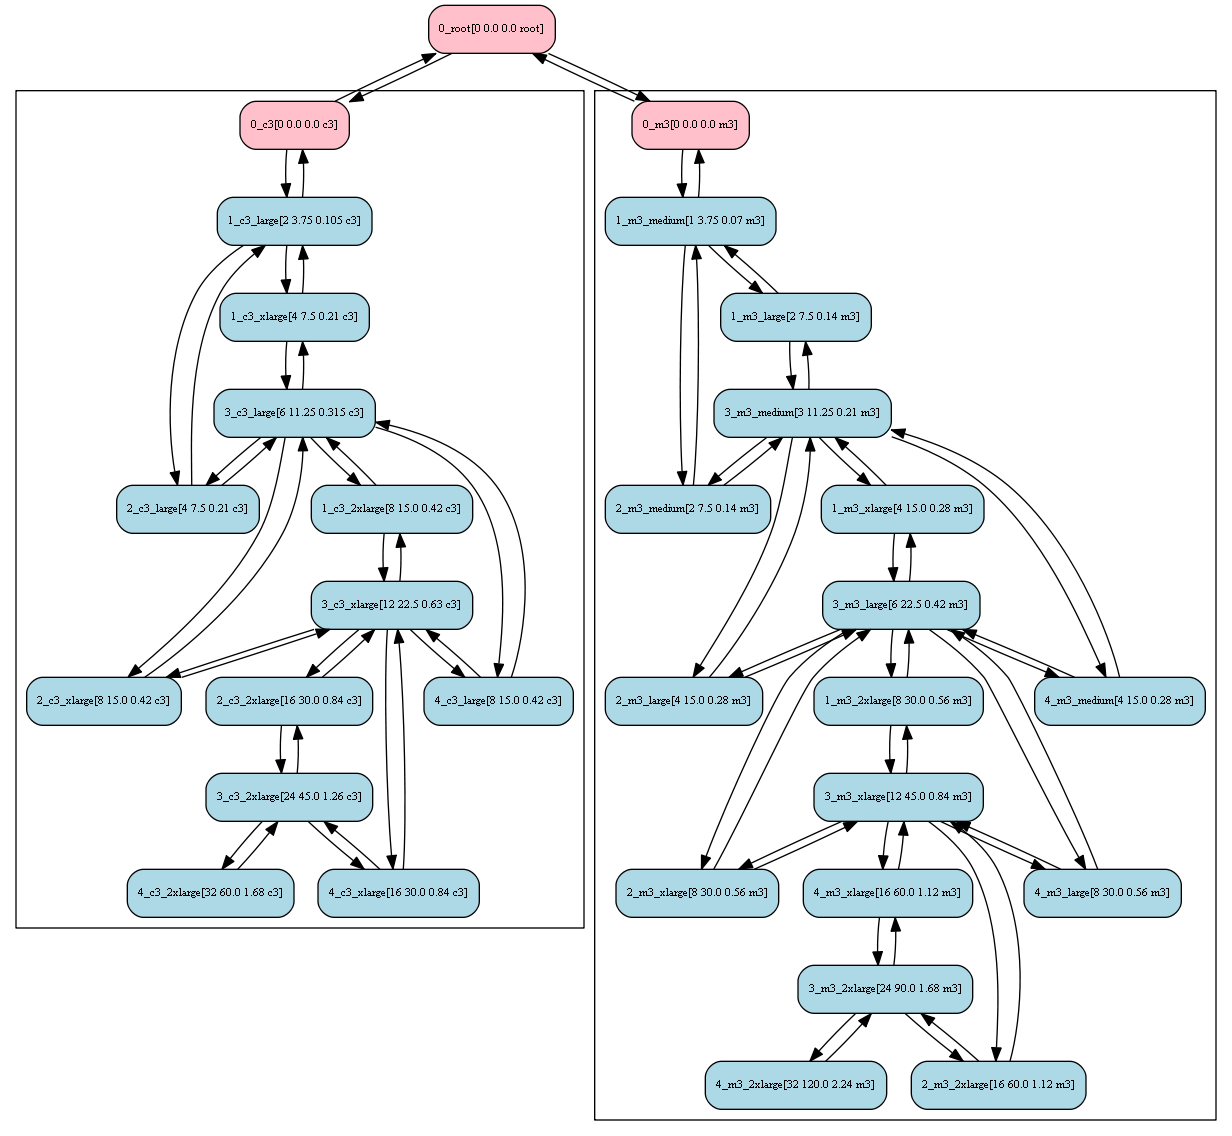
\includegraphics[scale=0.37]{img/exemplo_grafo_espaco_implantacao}
    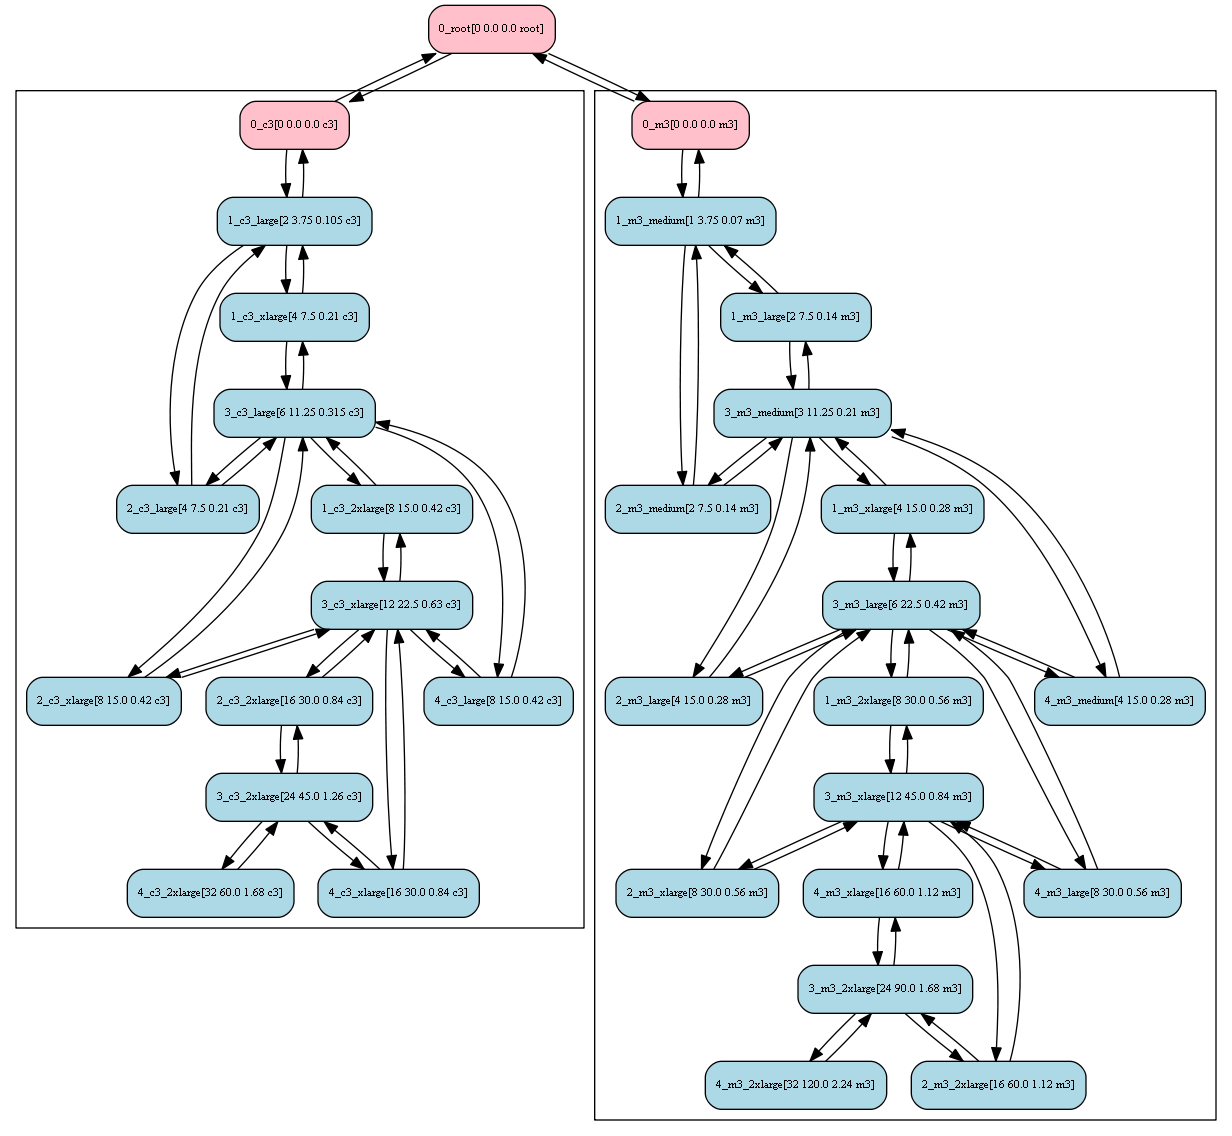
\includegraphics[width=\linewidth]{img/exemplo_grafo_espaco_implantacao}
  \end{center}
  \caption{\label{fig:depspace_real}Representação interna de um Espaço de Implantação no CloudCapacitor.}
\end{figure}

Como é possível ver na Figura~\ref{fig:depspace_real}, o Espaço de Implantação é 
representado internamente por um grafo direcionado onde arestas ligam duas 
Configurações para identificar as relações imediatas ``maior que'' e ``menor que'', 
conforme as definições da Seção~\ref{subsec:processo_niveis_capacidade}. 

CloudCapacitor separa o Espaço de Implantação em subgrafos, agrupando as
Configurações por Categoria de Máquinas Virtuais. Cada subgrafo é destinado às
Configurações cujo Tipo de Máquina pertença a uma determinada Categoria. O primeiro
nó, observado no topo do grafo, é o nó raiz e serve apenas para estabelecer a 
separação e permitir o trânsito entre as Categorias.

As classes \emph{DeploymentSpace} e \emph{DeploymentSpaceBuilder} implementam
a geração do Espaço de Implantação com base na relação de capacidade ou na relação
de preço entre as Configurações. O desenvolvedor pode optar pelo grafo por capacidade ou por preço no momento da
instanciação do objeto \emph{Capacitor}. Embora esse não seja o foco desta 
pesquisa, isso foi feito para que pudesse ser estudada a influência da formação 
do Espaço de Implantação na precisão e eficiência de custo das Heurísticas de 
Seleção. Esses resultados serão discutidos no Capítulo~\ref{chap:resultados}.

O Espaço de Implantação é a estrutura que dá suporte à navegação das Estratégias
sobre os diversos Níveis de Capacidade no momento em que devem ser escolhidas
as próximas Configurações a serem testadas. Suporta também a técnica de Inferência 
de Desempenho na identificação das relações de tamanho e/ou preço entre as 
Configurações nos pontos onde o Processo marca as Candidatas ou Rejeitadas, 
mostrando-se como um ponto chave para o sucesso do Processo de Avaliação.

A próxima seção descreve a implementação e o funcionamento das Estratégias de 
Avaliação e como o desenvolvedor pode criar sua própria Estratégia que melhor
supra suas necessidades de seleção de Configurações. 

\subsubsection{Estratégias de Avaliação}
\label{subsubsec:funcionamento_estrategias}
A Estratégia de Avaliação é responsável por aplicar uma Heurística de 
Seleção de Configurações nos momentos em que o Processo precisa navegar
pelo Espaço de Implantação. Assim, a cada momento em que um novo Nível 
de Capacidade deve ser escolhido, segundo o fluxo de ações previsto no 
Processo de Avaliação proposto, a Estratégia é invocada e age conforme 
a implementação da Heurística selecionada para a Avaliação 
(v. Seção~\ref{subsec:selecao_cenarios}).

CloudCapacitor fornece uma classe chamada \emph{Strategy} como uma implementação
padrão para as 9 Heurísticas descritas no Capítulo~\ref{chap:processo}. As
Figuras~\ref{fig:strategy_workload_code}~e~\ref{fig:strategy_capacity_code}
mostram o código fonte dos métodos de seleção de Carga de Trabalho e Nível
de Capacidade, respectivamente, da classe  \emph{Strategy}.

\begin{figure}[t]
  \begin{lstlisting}[language=Ruby,linewidth=\textwidth,xleftmargin=.04\textwidth, numbers=left]
  def select_workload( workload_list )
    case @wkl_approach
      when :pessimistic
        workload_list.first
      when :optimistic
        workload_list.last
      when :conservative
        workload_list[ workload_list.size / 2 ]
    end
  end
  \end{lstlisting}
  \caption{\label{fig:strategy_workload_code}Seleção de Carga de Trabalho na classe \emph{Strategy}.}
\end{figure}

\begin{figure}[t]
  \begin{lstlisting}[language=Ruby,linewidth=\textwidth,xleftmargin=.04\textwidth, numbers=left]
  def take_a_capacity_level_from( unexplored_levels )
    levels = unexplored_levels.keys
    return [] if levels.empty?
    case @cfg_approach
      when :pessimistic
        unexplored_levels.assoc( levels[-1] )
      when :optimistic
        unexplored_levels.assoc( levels[0] )
      when :conservative
        unexplored_levels.assoc( levels[levels.size / 2] )
    end
  end
  \end{lstlisting}
  \caption{\label{fig:strategy_capacity_code}Seleção de Nível de Capacidade na classe \emph{Strategy}.}
\end{figure}

Ambas as implementações são bastante simples. Para a seleção da Carga de Trabalho,
o método recebe como parâmetro a lista ordenada de Cargas informada à classe 
\emph{Capacitor}, como mostrado na linha 8 da Figura~\ref{fig:mincode}. O método 
então considera a abordagem especificada para a seleção de Cargas de Trabalho 
(Otimista, Conservadora ou Pessimista). Se a abordagem especificada é a Pessimista, 
o método retorna a primeira Carga da lista, que é a menor. Se a abordagem for a
Otimista, retorna a última Carga, que é a maior. Caso a abordagem seja a Conservadora,
será retornada uma Carga do meio da lista.

A implementação da seleção do próximo Nível de Capacidade é bem similar. O método
recebe uma lista de Níveis de Capacidade onde cada item é uma lista das Configurações
que pertencem ao Nível. O método então analisa a abordagem especificada para a
seleção de Configurações e, se a abordagem for a Pessimista, retorna a lista de 
Configurações do maior e último Nível de Capacidade. Se a abordagem for a Otimista, 
retorna as Configurações do primeiro Nivel, ou seja, o menor deles. Caso a abordagem
seja Conservadora, as Configurações retornadas serão as que compõem o Nível de 
Capacidade do meio da lista de Níveis.    

A combinação das abordagens de seleção para Cargas de Trabalho e Níveis de 
Capacidade nos métodos descritos corresponde às 9 Heurísticas apresentadas na
Seção~\ref{subsubsec:heuristicas}. Os experimentos realizados neste trabalho e 
apresentados no Capítulo~\ref{chap:resultados} foram todos executados com a 
implementação mostrada acima que, como será analisado, demonstra grande eficiência
na predição de desempenho para a Aplicação sob Teste avaliada.
 
Porém, caso se faça necessário atender especificidades da Aplicação sob Teste, 
é possível substituir essa implementação padrão trazida pela classe \emph{Strategy} 
por uma mais adequada aos objetivos do usuário. O relacionamento entre a classe 
\emph{Capacitor} e a Estratégia de Avaliação se dá conforme o padrão de projeto 
\emph{Strategy} \cite{gamma}, o que justifica a escolha 
do nome da classe e do conceito criado para a implementação das Heurísticas.

Assim, para que uma nova lógica de seleção de Cargas de Trabalho seja fornecida
ao CloudCapacitor, basta que o desenvolvedor implemente uma nova classe que estenda
\emph{Strategy} e sobrescreva o método \emph{select\_workload}. Analogamente,
para uma nova lógica de seleção de Níveis de Capacidade, a nova classe deve 
sobrescrever o método \emph{take\_a\_capacity\_level\_from}.

Essa flexibilidade oferecida pelo CloudCapacitor permite que seu uso seja 
customizado para uma ampla gama de Aplicações. Aliada essa característica à 
implementação de uma subclasse de \emph{DefaultExecutor}, customizando assim o 
controle da execução da Aplicação, CloudCapacitor se torna adaptável também ao
ambiente alvo dos testes, permitindo testes dos mais diversos.

Dando continuidade à descrição da implementação concreta do Processo de Avaliação,
a seção seguinte apresenta o retorno dos resultados obtidos pelo CloudCapacitor
após a execução da Avaliação.

\subsubsection{Resultado da Avaliação}
\label{subsubsec:funcionamento_resultado}

\begin{figure}[t]
 \begin{lstlisting}[linewidth=\textwidth,xleftmargin=.04\textwidth, numbers=left]
- 100
    m3.large
    c3.xlarge
    m3.2xlarge
- 200
    c3.xlarge
    m3.2xlarge
- 300
    c3.xlarge
    m3.2xlarge
- 400
    m3.2xlarge
  \end{lstlisting}
  \caption{\label{fig:resultado}Representação do retorno do resultado da execução do CloudCapacitor.}
\end{figure}

Durante toda a execução da Avaliação, CloudCapacitor segue colecionando as
Configurações marcadas como Candidatas, segundo a técnica de Inferência de 
Desempenho, para cada uma das Cargas de Trabalho especificadas como parâmetro de 
entrada. Ao final da execução, CloudCapacitor dispõe de uma lista de Cargas de Trabalho 
associadas cada qual a uma lista de Configurações Candidatas. Essa estrutura de
lista de listas é devolvida como retorno do método \emph{run\_for} da classe 
\emph{Capacitor}, cuja representação textual é ilustrada na Figura~\ref{fig:resultado}. 

Os dados retornados pelo \emph{Capacitor} podem então ser usados como base para escolha, por parte do usuário,
da Configuração mais barata que atende às diversas demandas esperadas para a 
sua aplicação implantada na nuvem.

Conclui-se assim a apresentação da implementação da biblioteca CloudCapacitor. A
seção a seguir mostra a implementação de um sistema de avaliação de capacidade 
que faz uso do CloudCapacitor e que foi usado neste trabalho para realizar os
experimentos de avaliação e analisar os seus resultados.

\section{Capacitor Web}
A fim de validar a implementação concreta do Processo através da biblioteca
CloudCapacitor, foi construída uma aplicação web, utilizando o \emph{framework} Ruby on Rails, que faz uso das funcionalidades oferecidas para a realização de testes de Avaliação de Capacidade em ambientes
de nuvem. A aplicação, denominada Capacitor Web, foi utilizada também
para a execução dos experimentos que fazem parte deste trabalho.

\begin{figure}[t]
  \begin{center}
    %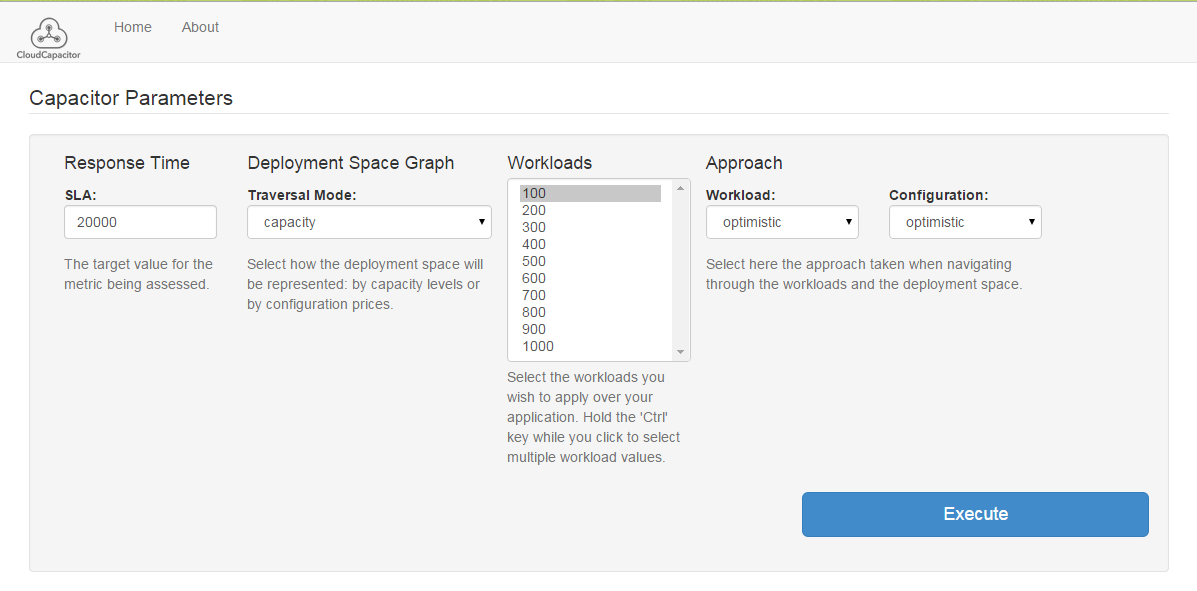
\includegraphics[scale=0.5]{img/CapacitorWeb_Frontpage}
    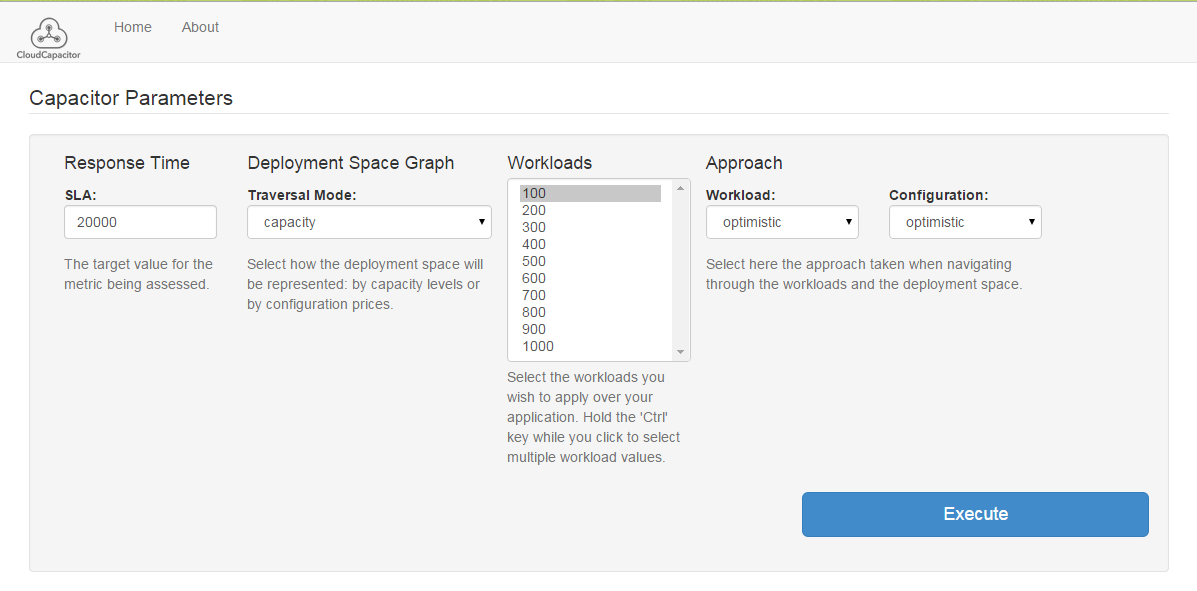
\includegraphics[width=\linewidth]{img/CapacitorWeb_Frontpage}
  \end{center}
  \caption{\label{fig:capacitor_web_front}Página inicial do Capacitor Web.}
\end{figure}

A Figura~\ref{fig:capacitor_web_front} mostra a tela inicial da aplicação, onde
o usuário tem a oportunidade de parametrizar a execução da Avaliação. O primeiro
campo permite a especificação do SLA que deve ser respeitado pela Aplicação para
que uma execução seja considerada bem sucedida. Em seguida, apresenta-se o campo
para seleção da representação do Espaço de Implantação, com opções de representação
por capacidade ou por preço.

Mais ao centro da tela está uma lista de valores para que o usuário selecione quais 
serão repassados ao CloudCapacitor como a lista de Cargas de Trabalho a serem impostas
sobre a Aplicação sob Teste. O usuário pode selecionar valores em qualquer ordem e mesmo
não adjacentes na lista.

Os últimos dois campos apresentam as opções de abordagens a serem usadas na seleção de
Cargas de Trabalho e Níveis de Capacidade. A combinação dessas duas abordagens forma a
Heurística de Seleção que a Estratégia de Avaliação usará nos momentos apropriados. As 
opções aqui são ``\emph{Optimistic}'', ``\emph{Conservative}'' e ``\emph{Pessimistic}''
para ambos os campos. Depois de selecionados os parâmetros, o usuário ordena a execução 
ao pressionar o botão presente na parte inferior da tela.

\begin{figure}[t]
  \begin{center}
    %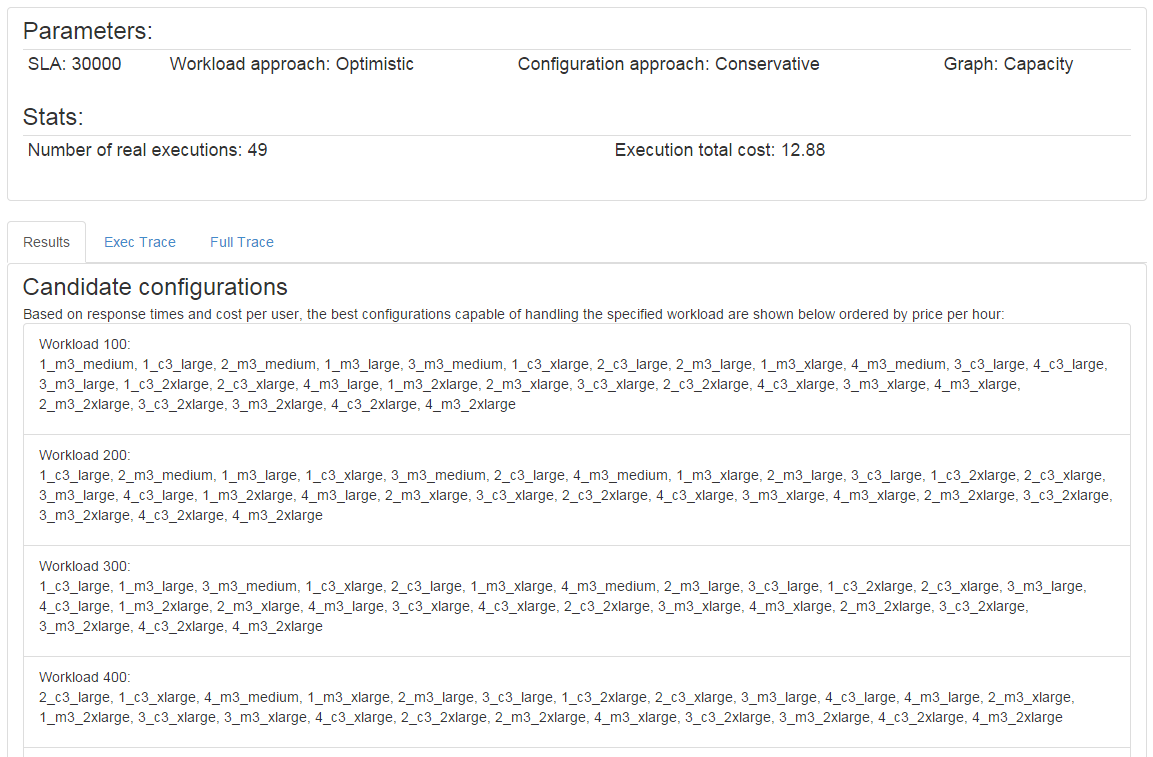
\includegraphics[scale=0.5]{img/CapacitorWeb_Results}
    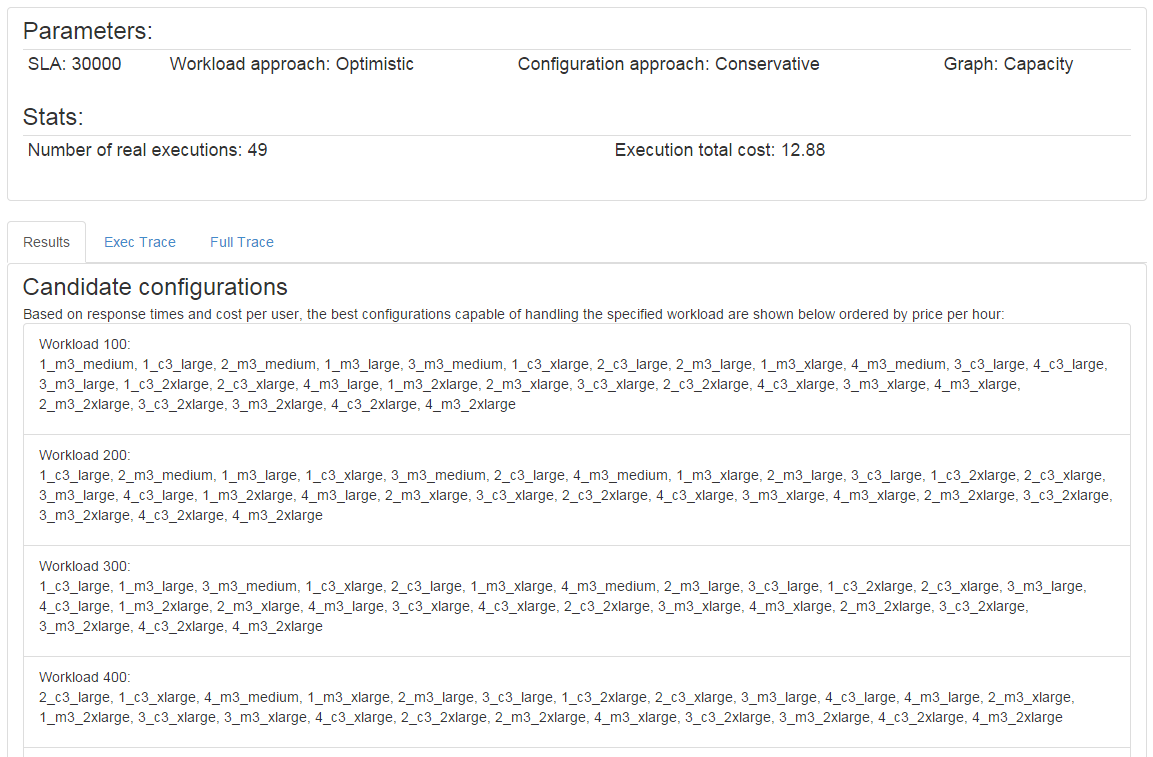
\includegraphics[width=\linewidth]{img/CapacitorWeb_Results}
  \end{center}
  \caption{\label{fig:capacitor_web_results}Página de Resultados do Capacitor Web.}
\end{figure}

Uma vez concluída a execução da Avaliação, o sistema apresenta ao usuário a tela
cuja imagem está na Figura~\ref{fig:capacitor_web_results}. Essa tela se divide
em duas grandes áreas, uma superior, fixa, e uma inferior, que, por sua vez, 
se subdivide em três partes, separadas conforme as abas que dividem a parte 
superior da inferior.

A parte superior mostra os dados passados como parâmetros pelo usuário na tela
inicial, para facilitar a análise dos resultados e sua comparação futura. Assim,
são exibidos o valor do SLA, as abordagens para Cargas de Trabalho e Níveis de 
Capacidade, formando a Heurística de Seleção utilizada, e o atributo usado para
geração do grafo que representa o Espaço de Implantação, isto é, capacidade ou
preço. Abaixo, são exibidos o número de execuções reais realizadas no ambiente
de nuvem alvo da Avaliação e o custo total por hora dessas execuções, com base
no preço definido pelo Provedor para as Configurações efetivamente utilizadas no 
teste. 
 
As abas da parte inferior ativam a visualização das informações complementares 
resultantes da execução. A primeira, com título ``Results'', exibe a saída 
retornada pela chamada ao método \emph{run\_for} da classe \emph{Capacitor} da 
biblioteca, conforme descrito na seção anterior. Essa saída é formada por um 
conjunto de valores de Cargas de Trabalho e, abaixo de cada um, uma lista com os 
nomes das Configurações consideradas como Candidatas para executar com sucesso a 
Aplicação sob aquela Carga.  

\begin{figure}[t]
  \begin{center}
    %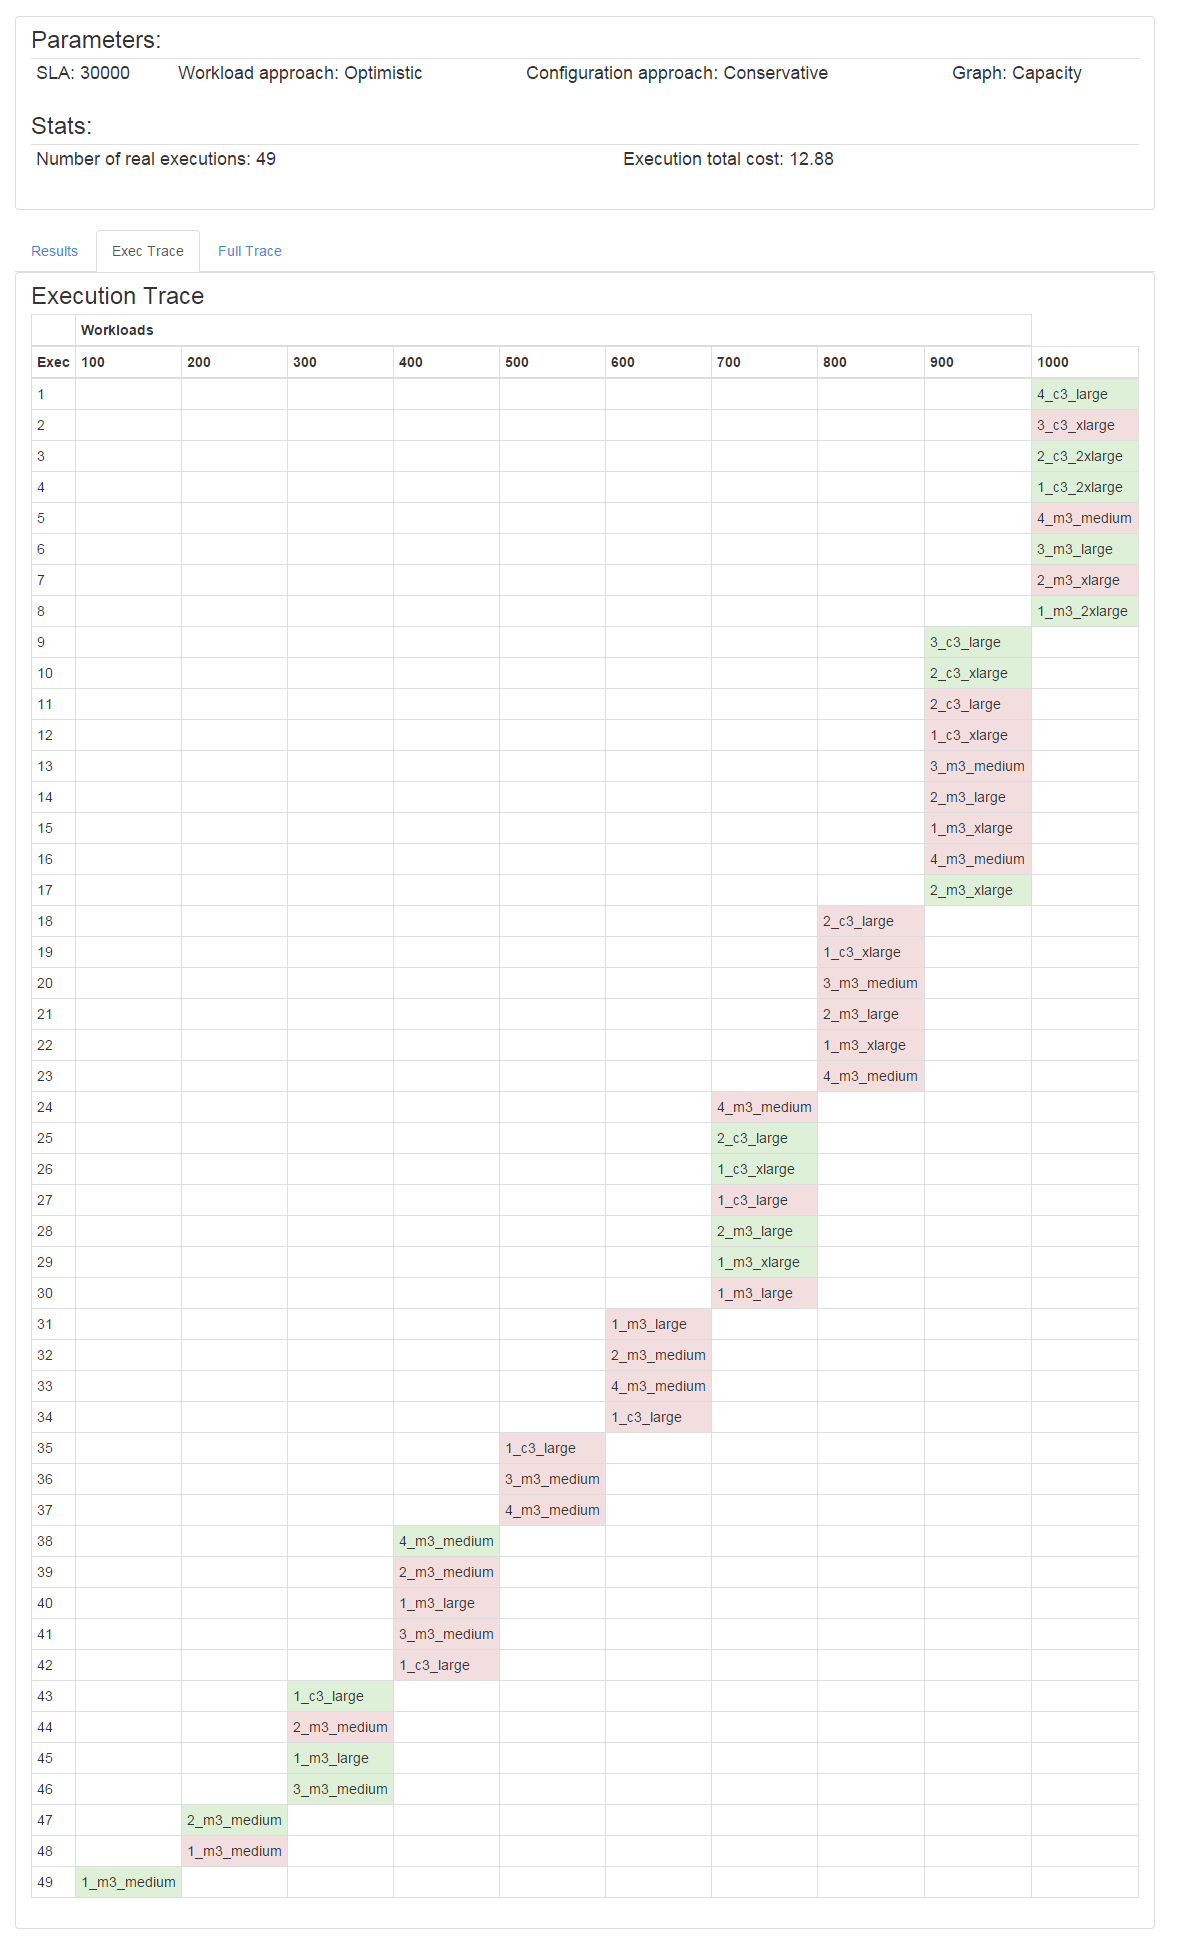
\includegraphics[scale=0.45]{img/CapacitorWeb_ExecutionTrace}
    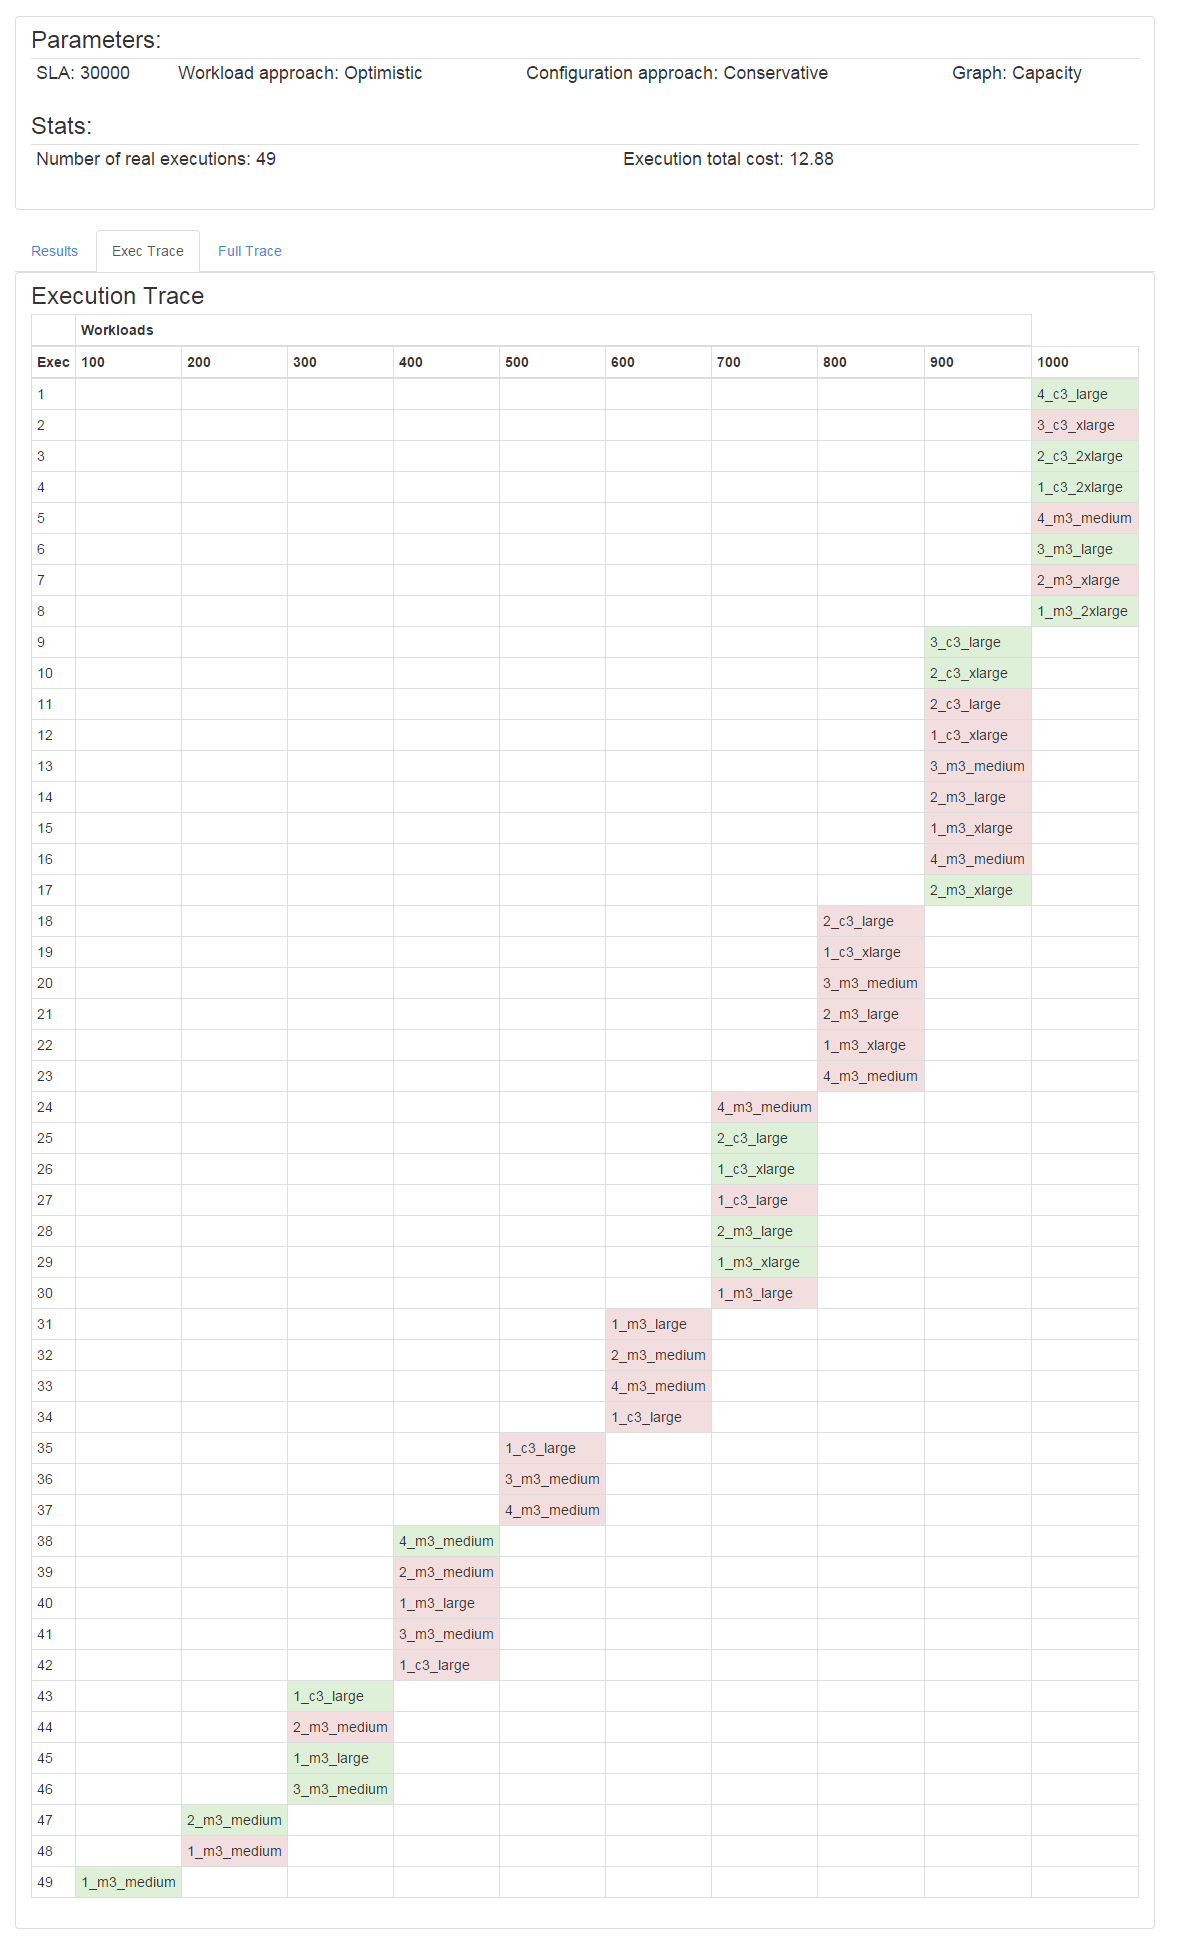
\includegraphics[width=\linewidth]{img/CapacitorWeb_ExecutionTrace}
  \end{center}
  \caption{\label{fig:capacitor_web_trace}Rastro de Execução do Capacitor Web.}
\end{figure}

A segunda aba da parte inferior da tela de resultados apresenta o título 
``Exec Trace'' e ativa a exibição dos dados de rastreamento da execução. Essa
visualização permite que o usuário analise a sequência de execuções reais da 
Aplicação sob Teste, apontando em que momento cada Carga de Trabalho foi aplicada
e qual Configuração foi usada para aferir o desempenho da Aplicação. A 
Figura~\ref{fig:capacitor_web_trace} mostra uma imagem dessa tela.

Os dados são exibidos em uma tabela cujas linhas apresentam a sequencia das 
execuções, identificadas pelo número presente na primeira coluna. Cada coluna da
tabela representa uma Carga de Trabalho e as células, que são a interceção entre
uma sequencia de execução e uma Carga, trazem um texto com o nome da Configuração 
utilizada naquela execução daquela Carga de Trabalho. As células que aparecem na 
cor esverdeada indicam as execuções onde o SLA foi satisfeito. De modo contrário, 
as células na cor avermelhada indicam as execuções onde a Aplicação não conseguiu 
desempenho suficiente para satisfazer o SLA.
 
\begin{figure}[t]
  \begin{center}
    %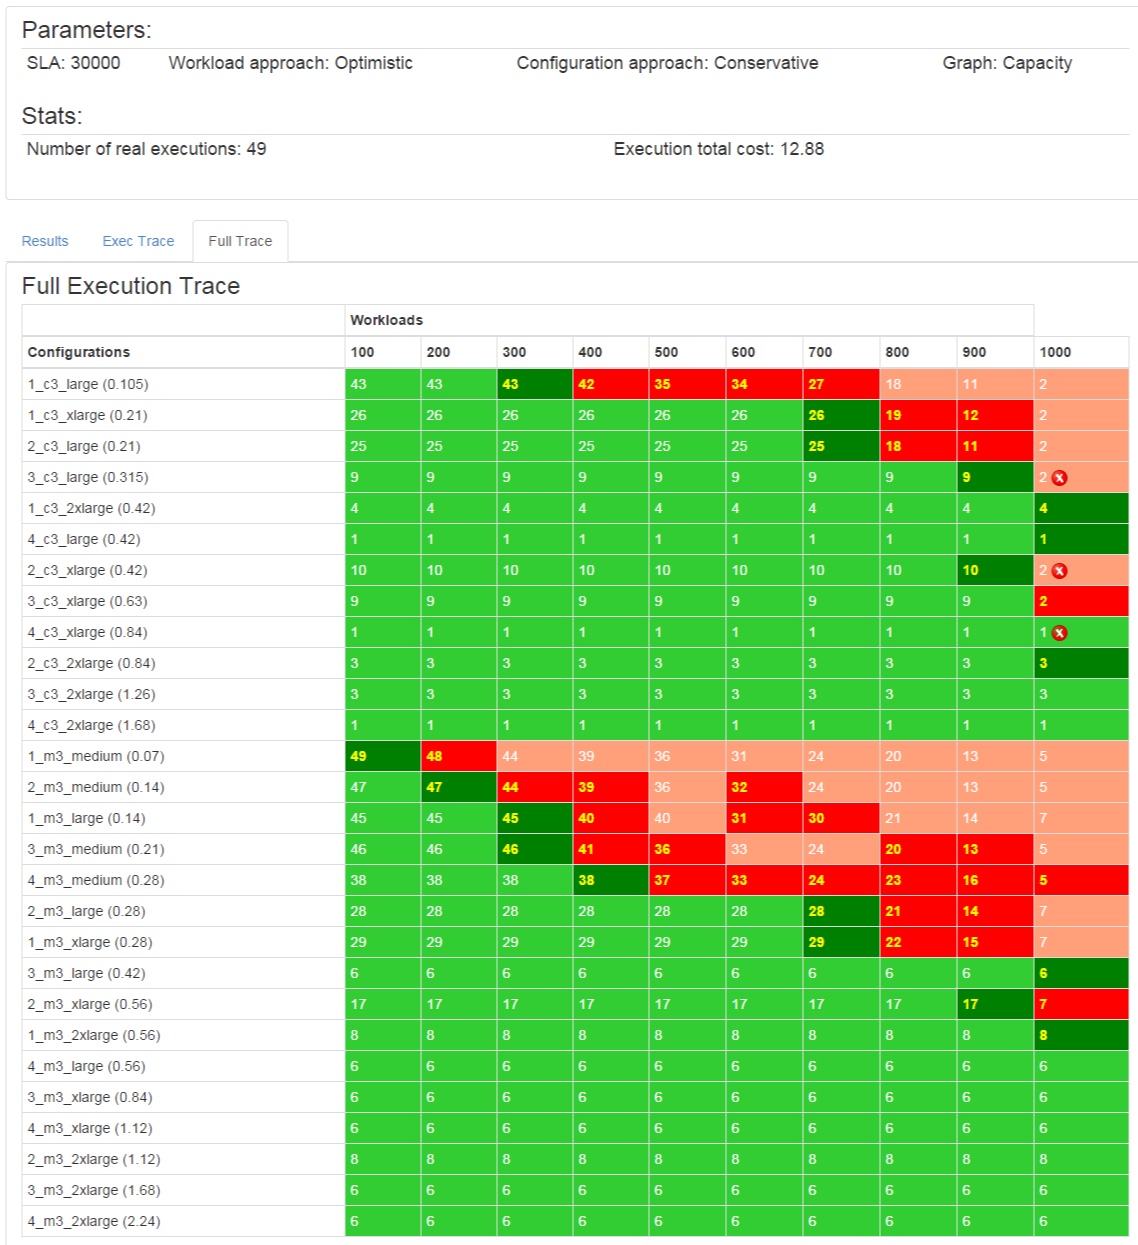
\includegraphics[scale=0.5]{img/CapacitorWeb_FullTrace}
    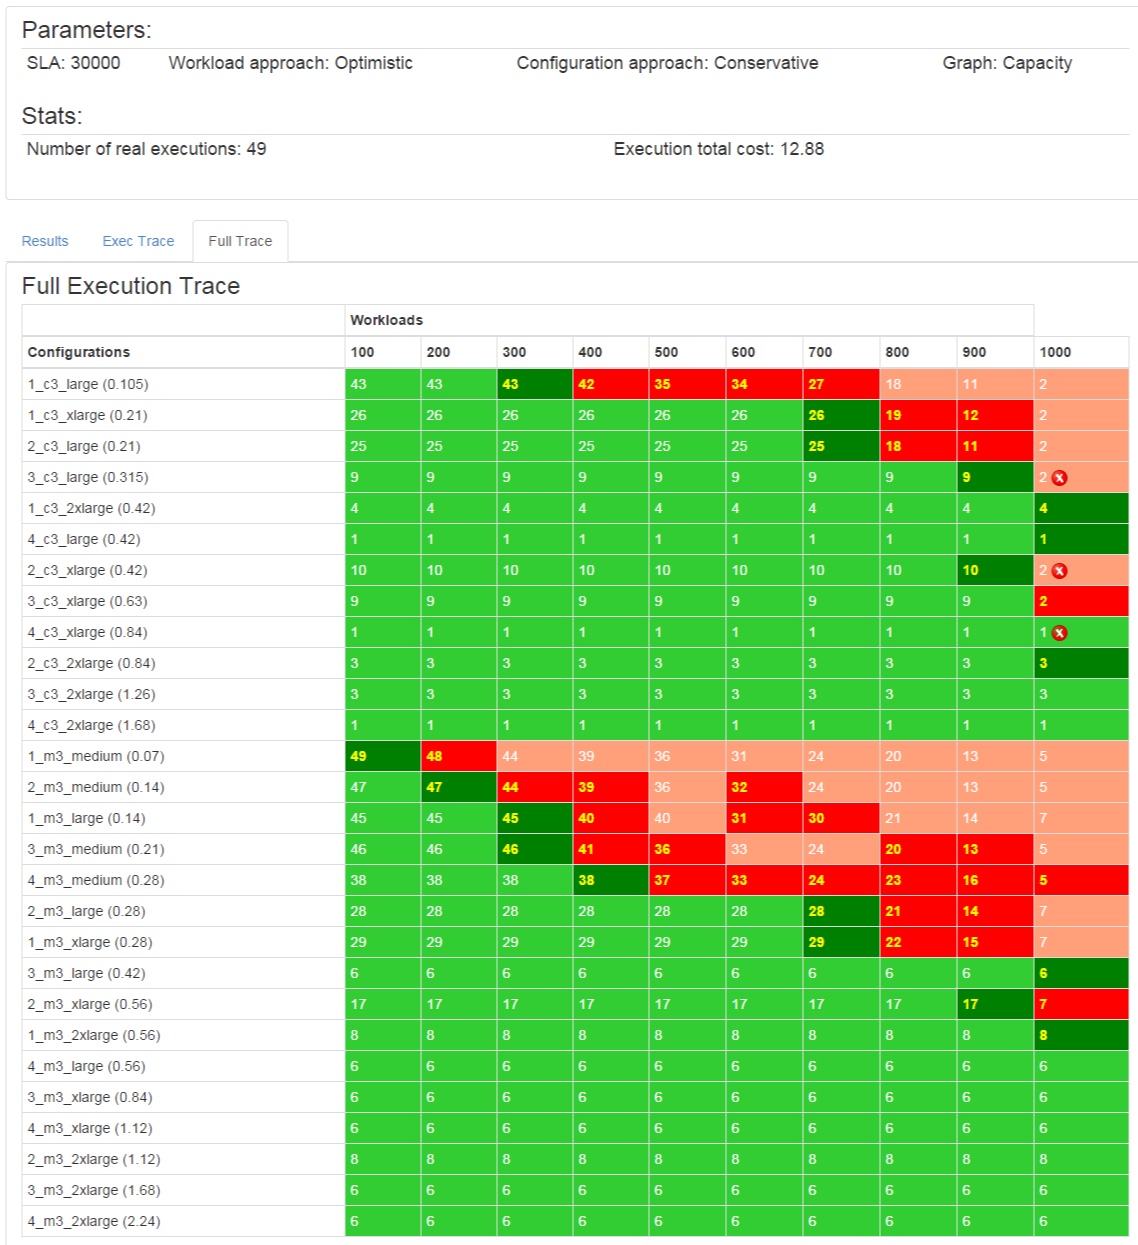
\includegraphics[width=\linewidth]{img/CapacitorWeb_FullTrace}
  \end{center}
  \caption{\label{fig:capacitor_web_fulltrace}Rastro Completo da Execução do Capacitor Web.}
\end{figure}

Por fim, a terceira aba, com o título ``Full Trace'', traz também uma tabela, 
esta com as colunas representando as Cargas de Trabalho e as linhas representando
as Configurações, como pode ser visto na Figura~\ref{fig:capacitor_web_fulltrace}. 
As células representam as execuções de cada Configuração em cada Carga de Trabalho 
e sua cor indica o sucesso ou fracasso em atender ao SLA.

Cada célula dessa tabela traz um número que identifica a execução real que levou
ao resultado representado pela cor da célula. As células dessa tabela podem aparecer
pintadas em quatro cores diferentes:

\begin{description}
  \item[Verde Escuro] \hfill \\ Execução real que satisfez o SLA
  \item[Verde Claro] \hfill \\ Predição de Configuração Candidata
  \item[Vermelho Escuro] \hfill \\ Execução real que não satisfez o SLA
  \item[Vermelho Claro] \hfill \\ Predição de Configuração Rejeitada
\end{description}

As células em cores claras são as Configurações para as quais não houve uma execução
real, mas cujo desempenho foi inferido. O número constante da célula indica qual
execução real levou o CloudCapacitor a marcar a Configuração como Candidata ou 
Rejeitada para a Carga de Trabalho em questão.

Quando são feitas essas predições de desempenho, em que o sucesso ou fracasso
da Configuração em satisfazer o SLA é inferido com base no desempenho de outra
Configuração, há a possibilidade de que a predição não tenha sido feita corretamente.
Quando essa situação acontece, o sistema faz uma marcação na célula com um pequeno
círculo vermelho com um ``\boldmath$\times$'' branco inscrito. A imagem da 
Figura~\ref{fig:capacitor_web_fulltrace} mostra essa marcação de erro de predição
na coluna referente à Carga de Trabalho de valor 1000 e linhas referentes às
Configurações ``3\_c3\_large'' e ``2\_c3\_xlarge'', onde a predição afirma erroneamente
que o SLA não seria satisfeito, e ``4\_c3\_xlarge'', onde a predição errou ao inferir 
que a Configuração conseguiria satisfazer o SLA. A explicação de como o Capacitor Web 
é capaz de saber se uma predição está correta ou não é dada no Capítulo~\ref{chap:resultados},
que detalha os experimentos realizados.

O rastreamento completo apresentado nessa tela permite a visualização da eficiência atingida
pela aplicação da Heurística nos testes de desempenho. Quanto maior a quantidade
de células pintadas em cor clara (quer sejam verdes ou vermelhas), maior o número
de predições, o que significa menor custo e menor tempo gasto na Avaliação. Do mesmo 
modo, quanto menor a presença dos círculos vermelhos indicadores de erro de predição,
maior a precisão alcançada pela técnica de Inferência de Desempenho ao prever quais
Configurações são capazes de atender cada Carga de Trabalho.

\section{Resumo}
Este capítulo apresentou a implementação concreta do Processo de Avaliação proposto no
Capítulo~\ref{chap:processo}, sob a forma de uma biblioteca a ser usada na criação de sistemas
mais completos destinados à avaliação de desempenho e capacidade de aplicações em nuvens IaaS.
Foram explicados os detalhes de programação necessários ao entendimento de como os conceitos vistos
foram concretizados em software, ao tempo em que foram descritos os passos envolvidos na 
customização das tarefas mais específicas ou que conferem flexibilidade ao Processo.

Foi mostrado ainda o sistema web criado para validação da implementação da biblioteca e para 
apoiar a execução dos experimentos realizados neste trabalho, com a descrição de sua interface de
entrada de dados e apresentação de resultados.

O Capítulo~\ref{chap:resultados}, a seguir, reporta os experimentos 
realizados, detalhando a metodologia utilizada, a Aplicação sob Teste e o Provedor escolhidos, as opções de implantação da aplicação avaliadas, e como foram realizadas as execuções para coleta de dados de desempenho. 
Além disso, serão analisados os resultados obtidos pela aplicação das 9 Heurísticas, 
comprovando e quantificando a eficiência do Processo de Avaliação de Capacidade proposto
e sua técnica de Inferência de Desempenho.
 
% ----------------------------------------------------------
